\documentclass[border=10pt]{standalone}

\usepackage{tikz}
\usepackage{tikzsymbols}
\usetikzlibrary{calc,patterns,shapes.geometric}

\def\centerarc[#1](#2)(#3:#4:#5){\draw[#1] ($(#2)+({#5*cos(#3)},{#5*sin(#3)})$) arc (#3:#4:#5);}

\begin{document}
	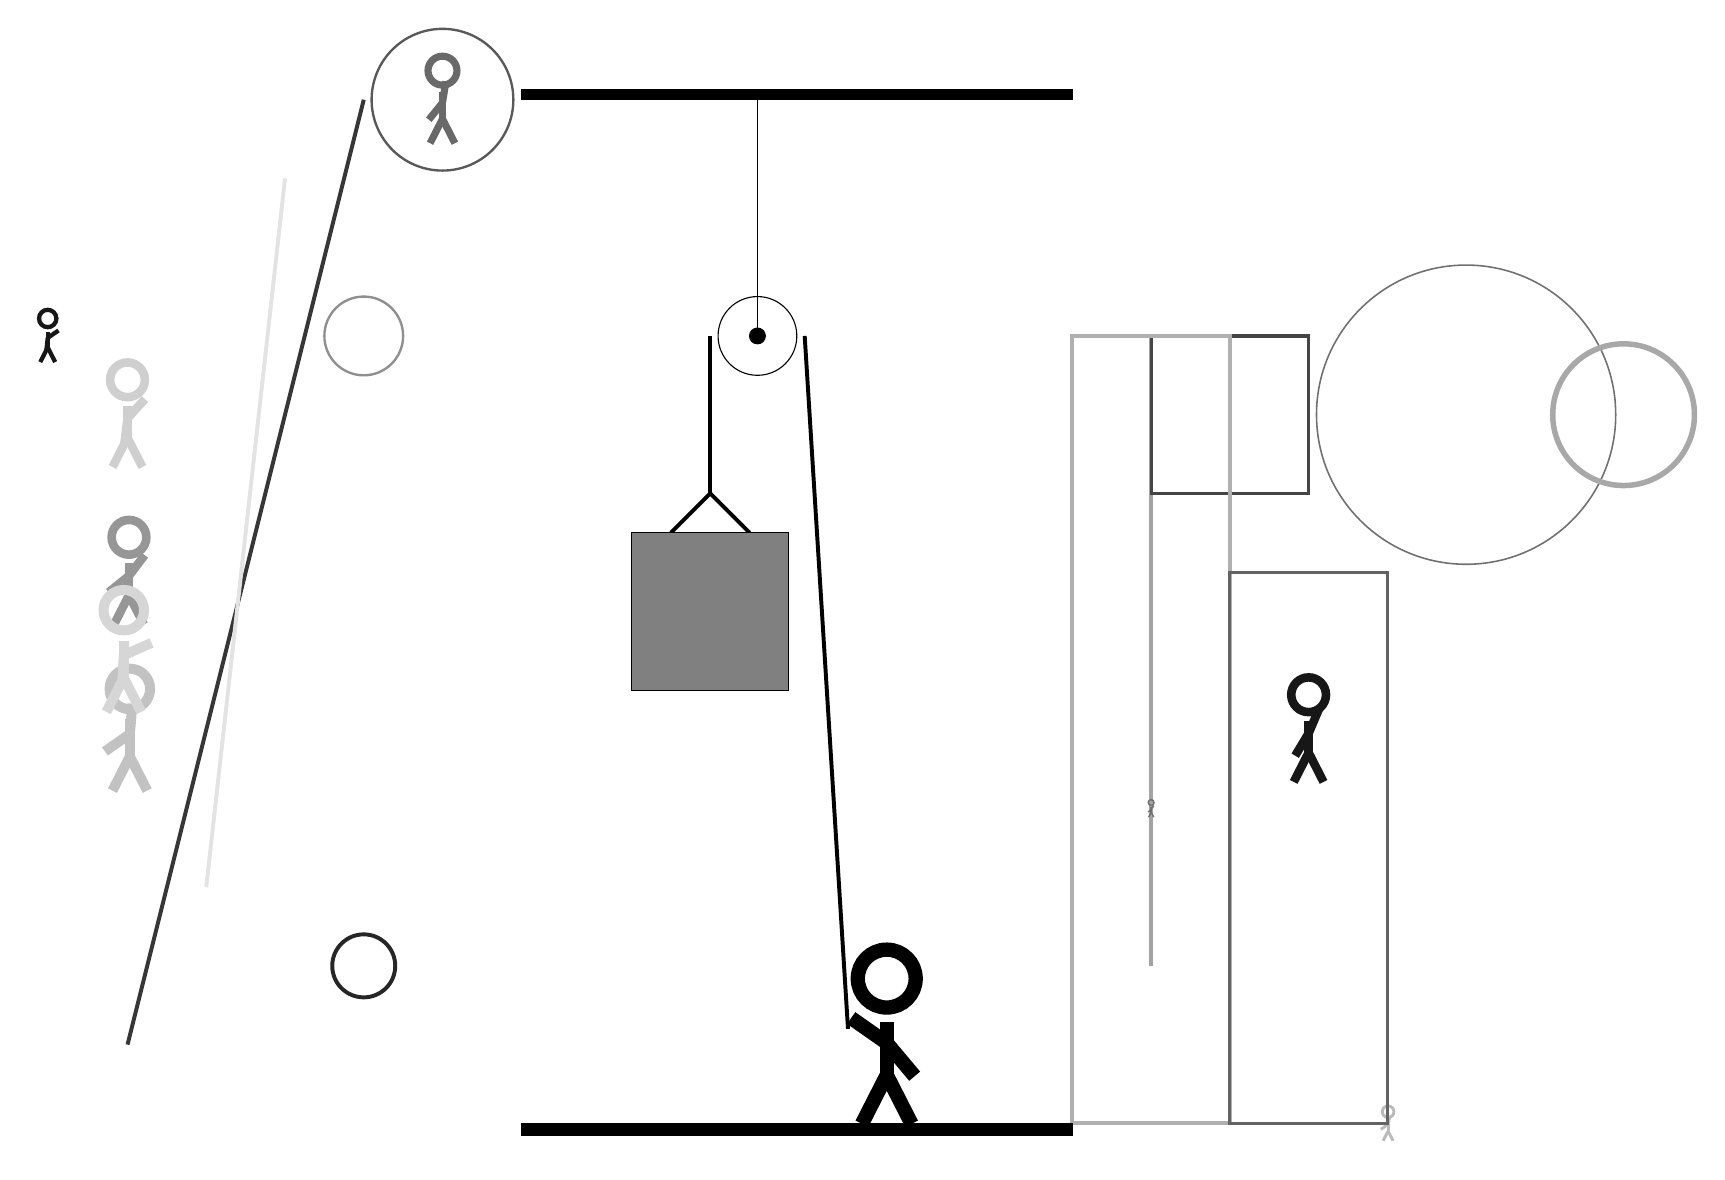
\begin{tikzpicture}
		%%%%% START %%%%%
		
		\draw[fill=black] (-2, 10) rectangle (5, 10.125);
		
		\draw (1, 7) circle (0.5);
		\draw[fill=black] (1, 7) circle (0.1);
		\draw (1, 10) -- (1, 7);
		
		\draw[line width=0.5mm] (-0.1, 4.5) -- (0.4, 5.0) -- (0.9, 4.5);
		\draw[fill=black!50] (-0.6, 4.5) rectangle (1.4, 2.5);
		
		\node[line width=0.5mm, color=black!24] at (-7, 2) {\Strichmaxerl[7][35][85]};
		
		\draw[line width=0.5mm, color=black!79](-4, 10) -- (-7, -2);
		\node[line width=0.6mm, color=black!27] at (9, -3) {\Strichmaxerl[2][33][78]};
		\node[line width=0.5mm, color=black!59] at (-3, 10) {\Strichmaxerl[5][51][81]};
		
		\draw[line width=0.5mm, color=black!36](6, 7) -- (6, -1);
		\draw[line width=0.4mm, color=black!73] (6, 5) rectangle (8, 7);
		\node[line width=0.7mm, color=black!41] at (-7, 4) {\Strichmaxerl[6][39][53]};
		\node[line width=0.5mm, color=black!91] at (-8, 7) {\Strichmaxerl[3][84][34]};
		\node[line width=0.2mm, color=black!19] at (-7, 6) {\Strichmaxerl[6][83][48]};
		
		\node[line width=0.6mm, color=black!16] at (-7, 3) {\Strichmaxerl[7][87][24]};
		\draw [line width=0.3mm, color=black!44](-4, 7) circle (0.5);
		\node[line width=0.4mm, color=black!56] at (6, 1) {\Strichmaxerl[1][48][50]};
		\draw [line width=0.5mm, color=black!85](-4, -1) circle (0.4);
		
		\node[line width=0.2mm, color=black!91] at (8, 2) {\Strichmaxerl[6][59][67]};
		\draw[line width=0.5mm, color=black!11](-6, 0) -- (-5, 9);
		\draw [line width=0.2mm, color=black!56](10, 6) circle (1.9);
		\draw[line width=0.5mm, color=black!31] (7, 7) rectangle (5, -3);
		\draw [line width=0.7mm, color=black!34](12, 6) circle (0.9);
		\draw [line width=0.3mm, color=black!65](-3, 10) circle (0.9);
		
		\draw[line width=0.4mm, color=black!61] (7, 4) rectangle (9, -3);
		
		\draw[line width=0.5mm] (0.4, 7) -- (0.4, 5.0);
		\centerarc[line width=0.5mm](1, 7)(0:180:0.6);
		\draw[line width=0.5mm](1.6, 7) -- (2.15, -1.8);
		
		\node at (2.6, -1.9) {\Strichmaxerl[10][-35][-50]};
		
		\draw[fill=black] (-2, -3) rectangle (5, -3.15);
		
		%%%%% END %%%%%
	\end{tikzpicture}
\end{document}